%%%%%%%%%%%%%%%%%%%%%%%%%%%%%%%%%%%%%%%%%
% Lachaise Assignment
% LaTeX Template
% Version 1.0 (26/6/2018)
%
% This template originates from:
% http://www.LaTeXTemplates.com
%
% Authors:
% Marion Lachaise & François Févotte
% Vel (vel@LaTeXTemplates.com)
%
% License:
% CC BY-NC-SA 3.0 (http://creativecommons.org/licenses/by-nc-sa/3.0/)
% 
%%%%%%%%%%%%%%%%%%%%%%%%%%%%%%%%%%%%%%%%%

%----------------------------------------------------------------------------------------
%	PACKAGES AND OTHER DOCUMENT CONFIGURATIONS
%----------------------------------------------------------------------------------------
\documentclass{article}

%%%%%%%%%%%%%%%%%%%%%%%%%%%%%%%%%%%%%%%%%
% Lachaise Assignment
% Structure Specification File
% Version 1.0 (26/6/2018)
%
% This template originates from:
% http://www.LaTeXTemplates.com
%
% Authors:
% Marion Lachaise & François Févotte
% Vel (vel@LaTeXTemplates.com)
%
% License:
% CC BY-NC-SA 3.0 (http://creativecommons.org/licenses/by-nc-sa/3.0/)
% 
%%%%%%%%%%%%%%%%%%%%%%%%%%%%%%%%%%%%%%%%%

%----------------------------------------------------------------------------------------
%	PACKAGES AND OTHER DOCUMENT CONFIGURATIONS
%----------------------------------------------------------------------------------------

\usepackage{amsmath,amsfonts,stmaryrd,amssymb} % Math packages
\usepackage{enumerate} % Custom item numbers for enumerations
\usepackage[ruled]{algorithm2e} % Algorithms
\usepackage[framemethod=tikz]{mdframed} % Allows defining custom boxed/framed environments
\usepackage{listings} % File listings, with syntax highlighting

\lstset{
	basicstyle=\ttfamily, % Typeset listings in monospace font
}

%----------------------------------------------------------------------------------------
%	DOCUMENT MARGINS
%----------------------------------------------------------------------------------------

\usepackage{geometry} % Required for adjusting page dimensions and margins

\geometry{
	paper=a4paper, % Paper size, change to letterpaper for US letter size
	top=2.5cm, % Top margin
	bottom=3cm, % Bottom margin
	left=2.5cm, % Left margin
	right=2.5cm, % Right margin
	headheight=14pt, % Header height
	footskip=1.5cm, % Space from the bottom margin to the baseline of the footer
	headsep=1.2cm, % Space from the top margin to the baseline of the header
}

%----------------------------------------------------------------------------------------
%	FONTS & LANGUAGE SETTINGS
%----------------------------------------------------------------------------------------

\usepackage{fontspec} % Required for font selection in XeLaTeX

%----------------------------------------------------------------------------------------
%	COMMAND LINE ENVIRONMENT
%----------------------------------------------------------------------------------------

\mdfdefinestyle{commandline}{
	leftmargin=10pt,
	rightmargin=10pt,
	innerleftmargin=15pt,
	middlelinecolor=black!50!white,
	middlelinewidth=2pt,
	frametitlerule=false,
	backgroundcolor=black!5!white,
	frametitle={Command Line},
	frametitlefont={\normalfont\sffamily\color{white}\hspace{-1em}},
	frametitlebackgroundcolor=black!50!white,
	nobreak,
}

% Define a custom environment for command-line snapshots
\newenvironment{commandline}{
	\medskip
	\begin{mdframed}[style=commandline]
	}{
	\end{mdframed}
	\medskip
}

%----------------------------------------------------------------------------------------
%	FILE CONTENTS ENVIRONMENT
%----------------------------------------------------------------------------------------

\mdfdefinestyle{file}{
	innertopmargin=1.6\baselineskip,
	innerbottommargin=0.8\baselineskip,
	topline=false, bottomline=false,
	leftline=false, rightline=false,
	leftmargin=2cm,
	rightmargin=2cm,
	singleextra={%
		\draw[fill=black!10!white](P)++(0,-1.2em)rectangle(P-|O);
		\node[anchor=north west]
		at(P-|O){\ttfamily\mdfilename};
		%
		\def\l{3em}
		\draw(O-|P)++(-\l,0)--++(\l,\l)--(P)--(P-|O)--(O)--cycle;
		\draw(O-|P)++(-\l,0)--++(0,\l)--++(\l,0);
	},
	nobreak,
}

% Define a custom environment for file contents
\newenvironment{file}[1][File]{ % Set the default filename to "File"
	\medskip
	\newcommand{\mdfilename}{#1}
	\begin{mdframed}[style=file]
	}{
	\end{mdframed}
	\medskip
}

%----------------------------------------------------------------------------------------
%	NUMBERED QUESTIONS ENVIRONMENT
%----------------------------------------------------------------------------------------

\mdfdefinestyle{question}{
	innertopmargin=1.2\baselineskip,
	innerbottommargin=0.8\baselineskip,
	roundcorner=5pt,
	nobreak,
	singleextra={%
		\draw(P-|O)node[xshift=1em,anchor=west,fill=white,draw,rounded corners=5pt]{%
			Question \theQuestion\questionTitle};
	},
}

\newcounter{Question} % Stores the current question number that gets iterated with each new question

% Define a custom environment for numbered questions
\newenvironment{question}[1][\unskip]{
	\bigskip
	\stepcounter{Question}
	\newcommand{\questionTitle}{~#1}
	\begin{mdframed}[style=question]
	}{
	\end{mdframed}
	\medskip
}

%----------------------------------------------------------------------------------------
%	WARNING TEXT ENVIRONMENT
%----------------------------------------------------------------------------------------

\mdfdefinestyle{warning}{
	topline=false, bottomline=false,
	leftline=false, rightline=false,
	nobreak,
	singleextra={%
		\draw(P-|O)++(-0.5em,0)node(tmp1){};
		\draw(P-|O)++(0.5em,0)node(tmp2){};
		\fill[black,rotate around={45:(P-|O)}](tmp1)rectangle(tmp2);
		\node at(P-|O){\color{white}\scriptsize\bf !};
		\draw[very thick](P-|O)++(0,-1em)--(O);
	}
}

% Define a custom environment for warning text
\newenvironment{warn}[1][Warning:]{
	\medskip
	\begin{mdframed}[style=warning]
		\noindent{\textbf{#1}}
	}{
	\end{mdframed}
}

%----------------------------------------------------------------------------------------
%	INFORMATION ENVIRONMENT
%----------------------------------------------------------------------------------------

\mdfdefinestyle{info}{%
	topline=false, bottomline=false,
	leftline=false, rightline=false,
	nobreak,
	singleextra={%
		\fill[black](P-|O)circle[radius=0.4em];
		\node at(P-|O){\color{white}\scriptsize\bf i};
		\draw[very thick](P-|O)++(0,-0.8em)--(O);
	}
}

% Define a custom environment for information
\newenvironment{info}[1][Info:]{
	\medskip
	\begin{mdframed}[style=info]
		\noindent{\textbf{#1}}
	}{
	\end{mdframed}
}

%----------------------------------------------------------------------------------------
%	ADDITIONAL PACKAGES
%----------------------------------------------------------------------------------------

\usepackage{graphicx}
\graphicspath{ {./Pics/} }
\usepackage[most]{tcolorbox}

\usepackage{xcolor}
\usepackage{booktabs}
\usepackage{siunitx}
\usepackage{placeins}

\usepackage{pgfplots}
\pgfplotsset{compat=1.18}
\usepackage{tikz}
 % Include the file specifying the document structure and custom commands

%----------------------------------------------------------------------------------------
%	ASSIGNMENT INFORMATION
%----------------------------------------------------------------------------------------

\title{\textbf{Computer Architecture Project Report - Dr. Jahangir}} % Title of the assignment

\author{\textbf{Nader Ahmadi - 403105674}} % Author name and email address

\date{\textbf{Sharif University of Technology - 2026}} % University, school and/or department name(s) and a date

%----------------------------------------------------------------------------------------

\begin{document}
	
	\maketitle % Print the title
	
	%----------------------------------------------------------------------------------------
	%	INTRODUCTION
	%----------------------------------------------------------------------------------------
	\vline
	
	
	\begin{tcolorbox}[colback=blue!5!white, colframe=blue!75!black, title=Notes]
		An \textbf{Apple M2 processor} was used to perform the experiments in this project.
	\end{tcolorbox}
	
	
	\setcounter{section}{0}
	\section{Part 1: Extracting Microarchitectural Fingerprints via Timing} % Unnumbered section
	In this section, we aim to investigate the following parameters:
	\begin{itemize}
		\item Cache levels and sizes (L1, L2, L3)
		\item Cache Line Size
		\item Degree of Set Associativity (N-way Set-Associative)
	\end{itemize}
	
	
	\subsection{Cache Level Sizes}
	
	In this part, we attempt to measure the latency of different cache levels using working dataset sizes ranging from $4\,\text{KB}$ to $64\,\text{MB}$. These sizes are doubled in each iteration to accurately detect the boundaries between different cache levels.
	
	First, an array of nodes is created, where the size of each node is $128$ bytes. The number of nodes at each test step is calculated by dividing the total data size by the size of a single node. The choice of $128$ bytes ensures complete filling of a cache line and prevents node misalignment across two separate cache blocks. A size of $64$ bytes was also tested, yielding identical results due to alignment maintenance.
	
	The connection between nodes is implemented using the \textbf{Pointer Chasing} technique, where each node contains the address of the next node, forming a sequential chain. Furthermore, to disable the hardware prefetcher and prevent the CPU from discovering access patterns, the \textbf{Fisher-Yates Shuffle} algorithm is employed. By traversing from the end of the array to the beginning, this algorithm shuffles the \texttt{next} pointers among various nodes.
	
	\begin{figure}[h]
		\centering
		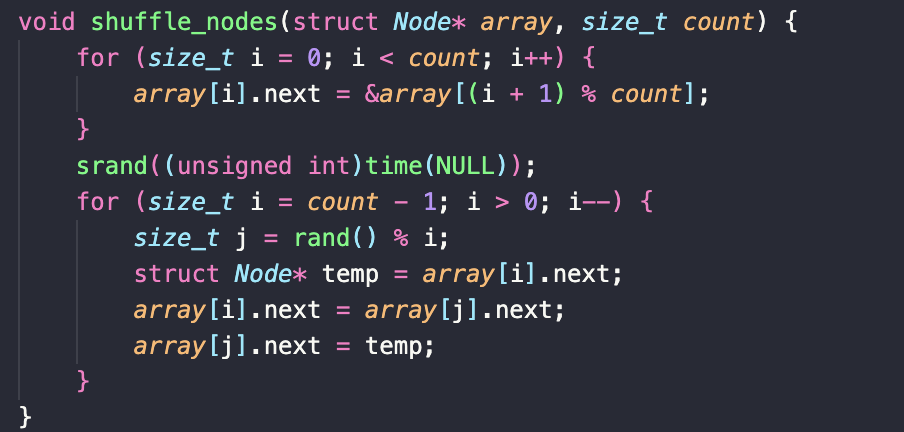
\includegraphics[width=0.5\textwidth]{1.png}
		\caption{Fisher-Yates Shuffle}
		\label{fig:}
	\end{figure}
	
	Since traversing the chain is extremely fast and makes execution time measurement difficult, we repeat the traversal 10 million times per loop iteration to produce a measurable execution time.
	
	The output of this step is presented below.
	
	\begin{figure}[h]
		\centering
		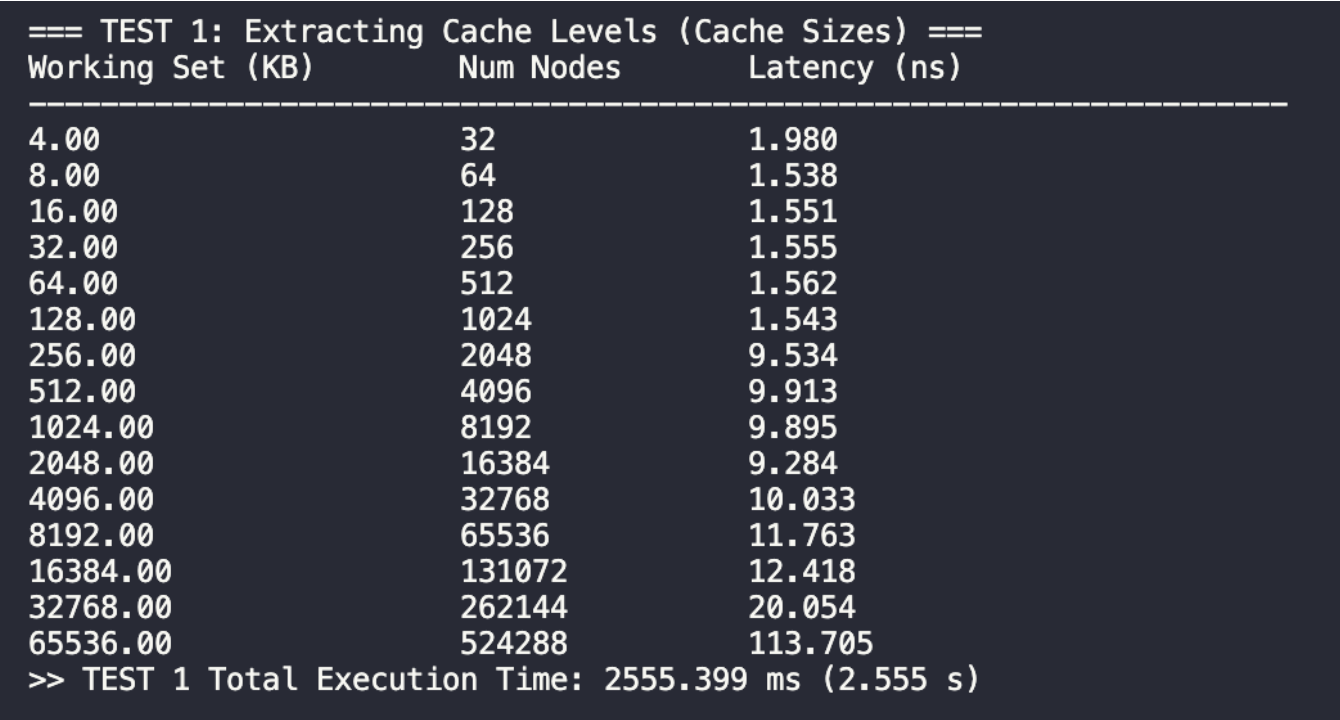
\includegraphics[width=0.6\textwidth]{T1.1_n.png}
		\caption{Cache Layer Size Test}
	\end{figure}
	
	\begin{figure}[htbp]
		\centering
		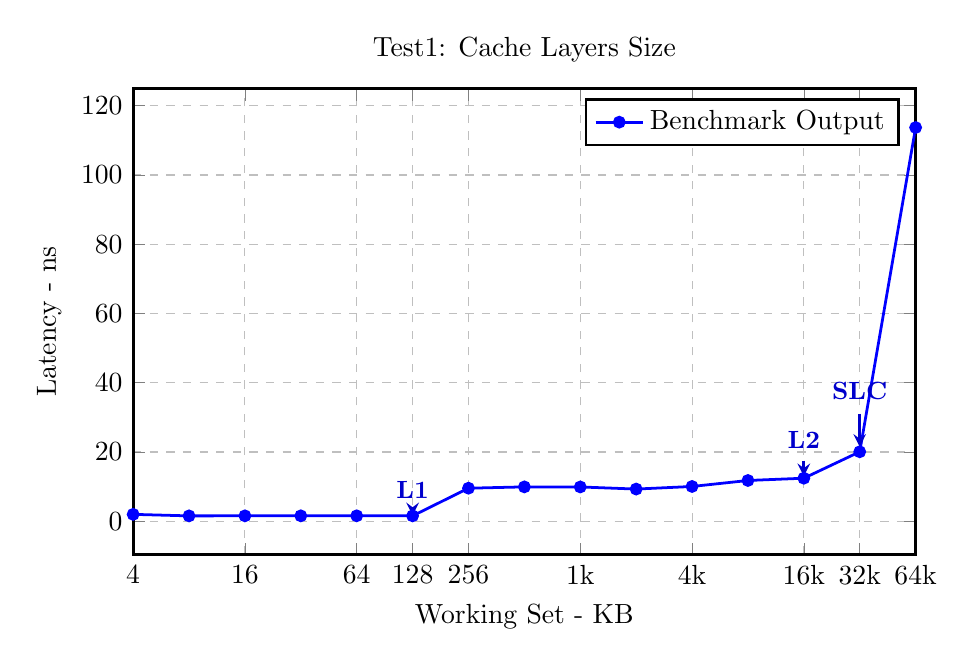
\begin{tikzpicture}
			\begin{axis}[
				title={Test1: Cache Layers Size},
				xlabel={Working Set - KB},
				ylabel={Latency - ns},
				xmode=log,
				log basis x={2},
				xmin=4, xmax=65536,
				xtick={4, 16, 64, 128, 256, 1024, 4096, 16384, 32768, 65536},
				xticklabels={4, 16, 64, 128, 256, 1k, 4k, 16k, 32k, 64k},
				xmajorgrids=true,
				ymajorgrids=true,
				grid style=dashed,
				width=0.95\textwidth,
				height=7.5cm,
				line width=1pt,
				mark size=1.8pt,
				]
				
				% Raw benchmark data
				\addplot[
				color=blue,
				mark=*,
				]
				coordinates {
					(4.00, 1.980)
					(8.00, 1.538)
					(16.00, 1.551)
					(32.00, 1.555)
					(64.00, 1.562)
					(128.00, 1.543)
					(256.00, 9.534)
					(512.00, 9.913)
					(1024.00, 9.895)
					(2048.00, 9.284)
					(4096.00, 10.033)
					(8192.00, 11.763)
					(16384.00, 12.418)
					(32768.00, 20.054)
					(65536.00, 113.705)
				};
				\legend{Benchmark Output}
				
				% 1. L1 Label at 128KB
				\node[anchor=south, font=\small\bfseries, color=blue!80!black] at (axis cs: 128, 3.5) {L1};
				\draw[->, >=stealth, blue!80!black] (axis cs: 128, 3.2) -- (axis cs: 128, 1.7);
				
				% 2. L2 Label at 16MB (16384KB)
				\node[anchor=south, font=\small\bfseries, color=blue!80!black] at (axis cs: 16384, 18) {L2};
				\draw[->, >=stealth, blue!80!black] (axis cs: 16384, 17.5) -- (axis cs: 16384, 13);
				
				% 3. SLC Label at 32MB (32768KB)
				\node[anchor=south, font=\small\bfseries, color=blue!80!black] at (axis cs: 32768, 32) {SLC};
				\draw[->, >=stealth, blue!80!black] (axis cs: 32768, 31) -- (axis cs: 32768, 21.5);
				
				% 4. RAM Label at last point (65536KB / 64MB)
				\node[anchor=east, font=\small\bfseries, color=red!80!black] at (axis cs: 65536, 113.705) {RAM \quad};
				
			\end{axis}
		\end{tikzpicture}
	\end{figure}
	
	\begin{tcolorbox}[colback=green!5!white, colframe=green!75!black, title=Results]
		As can be observed, up to 128 KB, the data fetch latency remains around \textbf{1.5 ns}, which corresponds to the \textbf{Level 1 (L1) Cache}. From 256 KB to 16 MB, the latency stays between \textbf{9.5 ns} and \textbf{12 ns}, representing the \textbf{Level 2 (L2) Cache}. Beyond that, a significant latency spike indicates main memory (RAM) access.\\
		\textbf{Note:} The M2 processor series does not feature a traditional L3 cache; instead, it incorporates a System Level Cache (SLC) shared across different functional blocks of the SoC. The capacity range of this cache is evaluated between 16 MB and 32 MB.\\
		
		Next, we compare our findings with the ground truth hardware values obtained via the following terminal command:
		\begin{center}
			\texttt{sysctl hw.perflevel0.l1dcachesize hw.perflevel0.l1icachesize hw.perflevel0.l2cachesize}
		\end{center}
		
		The output of this command is:
		\begin{center}
			\texttt{hw.perflevel0.l1dcachesize: 131072\\
				hw.perflevel0.l1icachesize: 196608\\
				hw.perflevel0.l2cachesize: 16777216}
		\end{center}
		which closely matches our experimental benchmark measurements.\\ 
		
		Occasionally, slight variations in the exact latency jump boundaries may occur across different runs. This happens because a portion of the L1 cache capacity may be occupied by background OS processes during execution.
	\end{tcolorbox}
	
	\subsection{Cache Line Size}
	
	In this section, the goal is to determine the exact size of each cache line (block) by varying the traversal stride (\textbf{Stride}). To perform this test, a data array of \textbf{32 MB} is allocated so that the dataset exceeds the L2 cache size and resides in \textbf{RAM}, making memory access latency clearly measurable.
	
	At each step, the total dataset size is divided by the \textbf{Stride} value to determine the number of nodes in the chain. Increasing the stride naturally reduces the total number of traversable nodes per cycle.
	
	\begin{figure}[h]
		\centering
		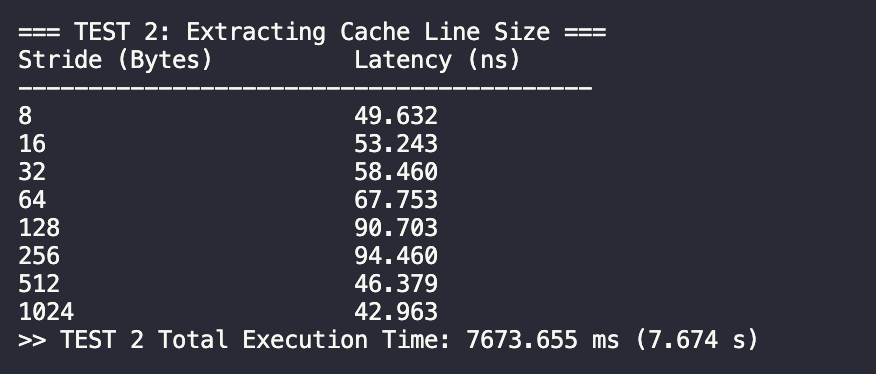
\includegraphics[width=0.6\textwidth]{T1.2_n.png}
		\caption{Cache Line Size Test}
		\label{fig:cache_line_size}
	\end{figure}
	
	\begin{figure}[htbp]
		\centering
		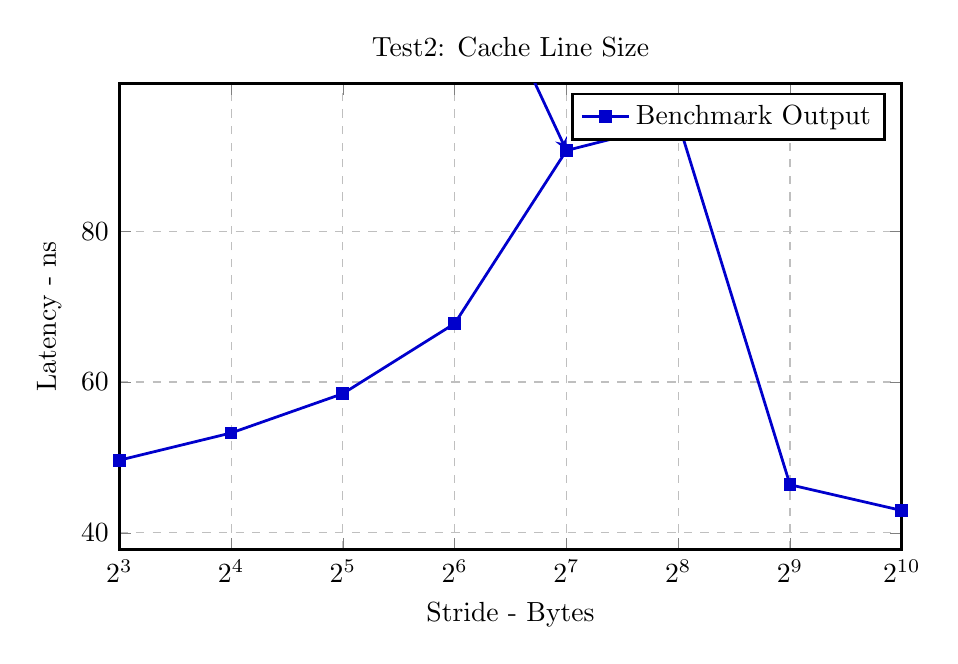
\begin{tikzpicture}
			\begin{axis}[
				title={Test2: Cache Line Size},
				xlabel={Stride - Bytes},
				ylabel={Latency - ns},
				xmode=log,
				log basis x={2},
				xmin=8, xmax=1024,
				xtick={8, 16, 32, 64, 128, 256, 512, 1024},
				xmajorgrids=true,
				ymajorgrids=true,
				grid style=dashed,
				width=0.95\textwidth,
				height=7.5cm,
				line width=1pt,
				mark size=1.8pt,
				]
				
				% Test 2 Data
				\addplot[
				color=blue!80!black,
				mark=square*,
				]
				coordinates {
					(8, 49.632)
					(16, 53.243)
					(32, 58.460)
					(64, 67.753)
					(128, 90.703)
					(256, 94.460)
					(512, 46.379)
					(1024, 42.963)
				};
				\legend{Benchmark Output}
				
				\node[anchor=south east, font=\small\bfseries, color=blue!80!black] at (axis cs: 90, 105) {$2^7 = 128 \text{ Bytes}$ (90.70 ns)};
				\draw[->, >=stealth, line width=1pt, color=blue!80!black] (axis cs: 100, 102) -- (axis cs: 128, 90.703);
				
			\end{axis}
		\end{tikzpicture}
	\end{figure}
	
	\begin{tcolorbox}[colback=green!5!white, colframe=green!75!black, title=Results]
		As shown in Figure~\ref{fig:cache_line_size}, a steep jump in access latency occurs at a \textbf{stride of 128 bytes}. Thus, we can conclude that the \textbf{Cache Line Size} is \textbf{128 bytes}. The decrease in latency at larger strides (256 bytes and above) is attributed to the drastic reduction in total node count, which significantly decreases total memory accesses per run.
		
		To verify this result, the following command was executed in the terminal:
		
		\begin{center}
			\texttt{sysctl hw.cachelinesize}
		\end{center}
		
		The command returned:
		\begin{center}
			\texttt{hw.cachelinesize: 128}
		\end{center}
		confirming the accuracy of our benchmark observation.
	\end{tcolorbox}
	
	
	\subsection{Set Associativity}
	
	In this section, the objective is to determine the number of cache ways (\textbf{Ways}) that can simultaneously map to a specific set (\textbf{Set}) in the cache. To achieve this, data points are selected at a constant offset of $16\,\text{KB}$ apart, ensuring that all selected addresses map to the exact same cache set.
	
	By incrementally increasing the number of mapped addresses from $1$ to $16$, we evaluate the capacity of that set. As long as the number of data items does not exceed the hardware set associativity, all items fit within the set, maintaining minimal latency. However, once set capacity is exceeded, additional items trigger \textbf{Conflict Misses}, evicting existing lines and causing a distinct latency spike that reveals the exact degree of associativity.
	
	The benchmark output for this step is as follows:
	
	\begin{figure}[h]
		\centering
		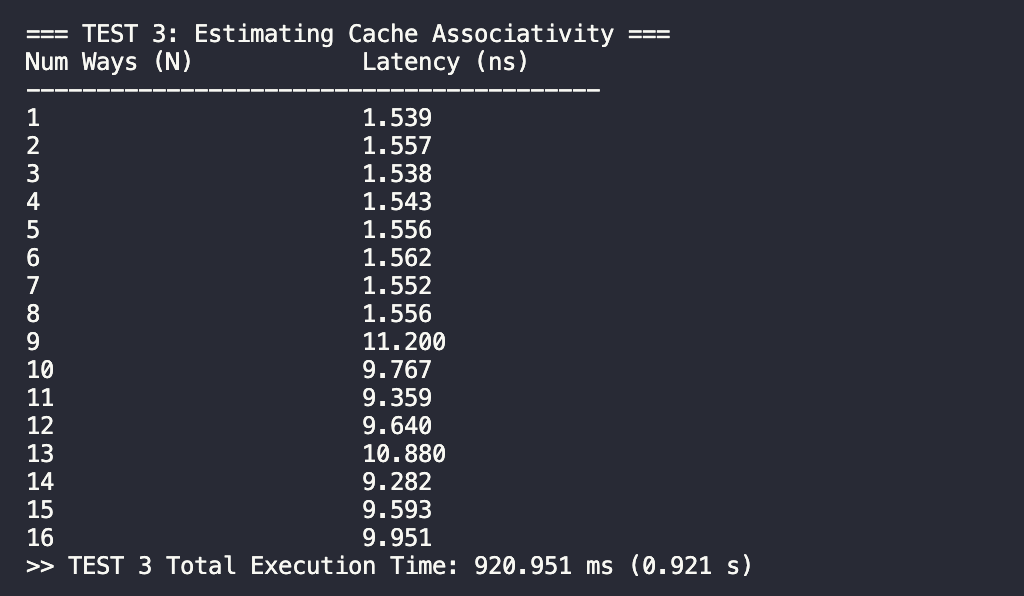
\includegraphics[width=0.6\textwidth]{T1.3_n.png}
		\caption{Set Associativity Test}
	\end{figure}
	
	\begin{figure}[htbp]
		\centering
		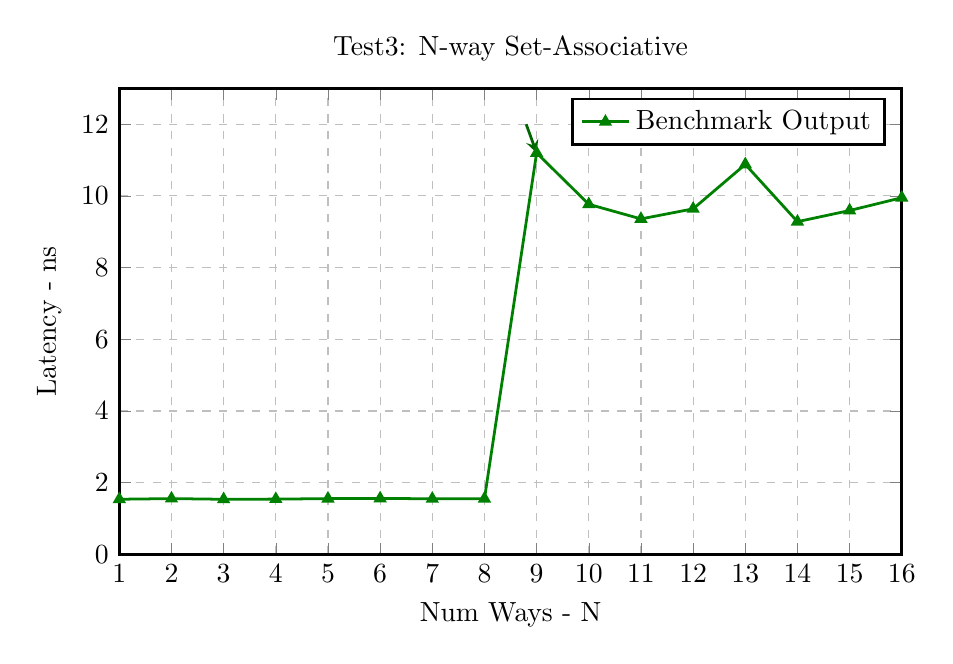
\begin{tikzpicture}
			\begin{axis}[
				title={Test3: N-way Set-Associative},
				xlabel={Num Ways - N},
				ylabel={Latency - ns},
				xmin=1, xmax=16,
				ymin=0, ymax=13,
				xtick={1, 2, 3, 4, 5, 6, 7, 8, 9, 10, 11, 12, 13, 14, 15, 16},
				xmajorgrids=true,
				ymajorgrids=true,
				grid style=dashed,
				width=0.95\textwidth,
				height=7.5cm,
				line width=1pt,
				mark size=1.8pt,
				]
				
				% Test 3 Data
				\addplot[
				color=green!50!black,
				mark=triangle*,
				]
				coordinates {
					(1, 1.539)
					(2, 1.557)
					(3, 1.538)
					(4, 1.543)
					(5, 1.556)
					(6, 1.562)
					(7, 1.552)
					(8, 1.556)
					(9, 11.200)
					(10, 9.767)
					(11, 9.359)
					(12, 9.640)
					(13, 10.880)
					(14, 9.282)
					(15, 9.593)
					(16, 9.951)
				};
				\legend{Benchmark Output}
				
				\draw[->, >=stealth, line width=1pt, color=green!40!black] (axis cs: 8.8, 12.0) -- (axis cs: 9, 11.200);
				
			\end{axis}
		\end{tikzpicture}
	\end{figure}
	
	\begin{tcolorbox}[colback=green!5!white, colframe=green!75!black, title=Results]
		As seen in the graph, a sudden spike in latency occurs at $N = 9$. We can therefore conclude that the processor features an \textbf{8-way set-associative L1 cache}. While official technical documentation from Apple regarding set associativity is limited, standard microarchitectural literature and LLM architectural references confirm that the Apple Silicon L1 Data Cache is indeed 8-way set-associative.
	\end{tcolorbox}
	
	\vspace{2cm}
	\section{Part 2: Reading Hardware Performance Counters}
	
	\begin{tcolorbox}[colback=blue!5!white, colframe=blue!75!black, title=Notes]
		Since the profiling tools mentioned in the generic project description were not directly available for macOS, we utilized \textbf{Xcode Instruments}. This tool allows detailed monitoring of CPU microarchitectural hardware events.
		To profile hardware performance counters, the target executable was attached within Instruments, adding custom event profiling configurations. The profiling session output is saved in the native \textbf{Trace} format.
	\end{tcolorbox}
	
	The benchmark executable developed in Part 1 was profiled using this setup. The extracted microarchitectural metrics are summarized in the table below:
	
	\begin{table}[htbp]
		\centering
		\caption{Microarchitecture Metrics Extracted from Xcode Instruments for Process (Samples: 141,538)}
		\label{tab:microarchitecture_metrics_full}
		\begin{tabular}{llrr}
			\toprule
			\textbf{Microarchitectural Metric} & \textbf{Hardware Event} & \textbf{Total Count} & \textbf{Calculated Rate / Ratio} \\
			\midrule
			Total Executed Instructions & \texttt{INST\_ALL} & 6,443,573,748 & 100.00\% \\
			Total CPU Clock Cycles & \texttt{Cycles} & 25,523,723,774 & -- \\
			\textbf{Execution Efficiency (IPC)} & \texttt{INST\_ALL / Cycles} & -- & \textbf{0.2525} ($\text{CPI} = 3.96$) \\
			\midrule
			L1 Data Cache Miss (Load) & \texttt{L1D\_CACHE\_MISS\_LD} & 295,389,509 & -- \\
			L1 Data Cache Miss (Store) & \texttt{L1D\_CACHE\_MISS\_ST} & 23,571,344 & -- \\
			\textbf{Total L1 Data Cache Misses} & \texttt{L1D\_CACHE\_MISS (Total)} & 318,960,853 & \textbf{4.95\%} (of total instructions) \\
			\midrule
			L1 Data TLB Accesses & \texttt{L1D\_TLB\_ACCESS} & 3,533,290,451 & -- \\
			\textbf{L1D Data TLB Misses} & \texttt{L1D\_TLB\_MISS} & 163,779,190 & \textbf{4.64\%} (TLB Miss Rate) \\
			\midrule
			Branch Instructions & \texttt{INST\_BRANCH} & 1,811,420,549 & 28.11\% (of total instructions) \\
			\textbf{Branch Mispredictions} & \texttt{BRANCH\_MISPRED\_NONSPEC} & 18,873 & \textbf{0.0010\%} (Misprediction Rate) \\
			\midrule
			\textbf{Profiling Resolution} & \texttt{\# Samples} & 141,538 & \textbf{$\approx 10,011$ Hz} (Samples/sec) \\
			\bottomrule
		\end{tabular}
	\end{table}
	
	The breakdown of function execution times is detailed below:
	
	\begin{table}[htbp]
		\centering
		\caption{Function Execution Time Distribution (Time Profiler Breakdown)}
		\label{tab:time_profiler_breakdown}
		\begin{tabular}{lrrr}
			\toprule
			\textbf{Benchmark Function} & \textbf{Total Time (Weight)} & \textbf{Self Time} & \textbf{\% of Total Runtime} \\
			\midrule
			\texttt{run\_cache\_line\_test} & 10.52 s & 10.34 s & \textbf{74.4\%} \\
			\texttt{run\_cache\_size\_test} & 2.67 s & 2.63 s & \textbf{18.9\%} \\
			\texttt{run\_associativity\_test} & 948.20 ms & 948.10 ms & \textbf{6.7\%} \\
			\midrule
			\textbf{Total Execution Time} & \textbf{14.14 s} & -- & \textbf{100.0\%} \\
			\bottomrule
		\end{tabular}
	\end{table}
	
	\begin{figure}[h]
		\centering
		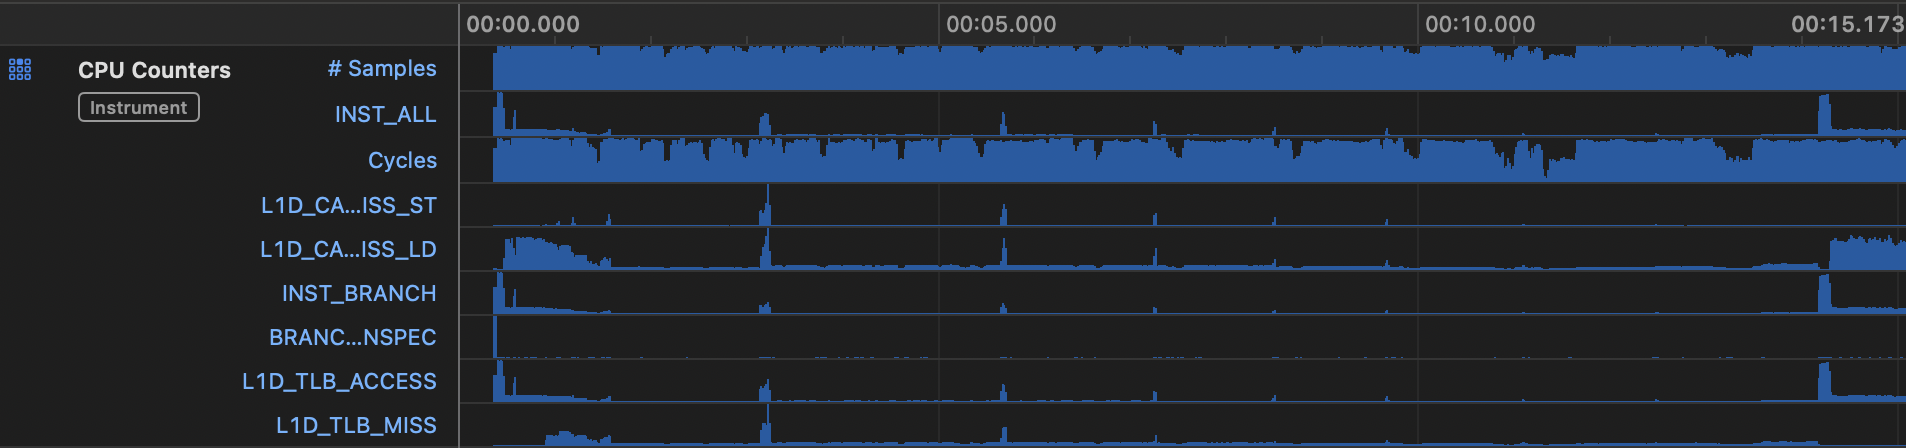
\includegraphics[width=0.75\textwidth]{Instruments_res.png}
		\caption{Overall Program Execution Timeline in Xcode Instruments}
	\end{figure}
	
	\subsection{Correlating Profiling Data with Part 1}
	We now analyze the individual timeline phases:
	
	\begin{figure}[h]
		\centering
		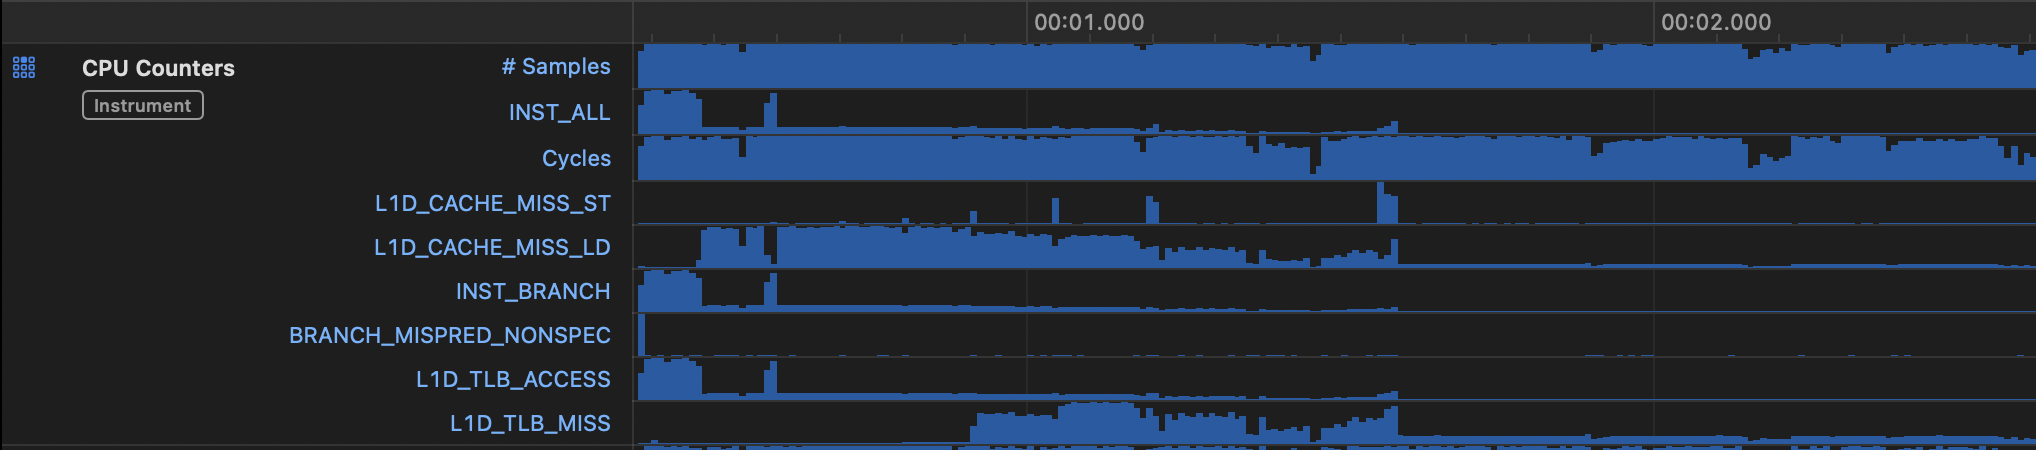
\includegraphics[width=0.75\textwidth]{T2.1.png}
		\caption{Timeline for Cache Layer Size Test}
	\end{figure}
	\FloatBarrier
	
	As observed, L1 data cache misses remain low initially. However, as dataset sizes increase beyond L1 bounds, miss counts experience a sharp surge, perfectly aligning with the findings in Part 1. Furthermore, towards the end of this test phase, miss density decreases. This occurs because at large array sizes (e.g., \textbf{16 MB, 32 MB}), each cache miss incurs a significant RAM latency delay, stalling the processing pipeline and resulting in fewer total misses generated per unit of time.
	
	\begin{figure}[h]
		\centering
		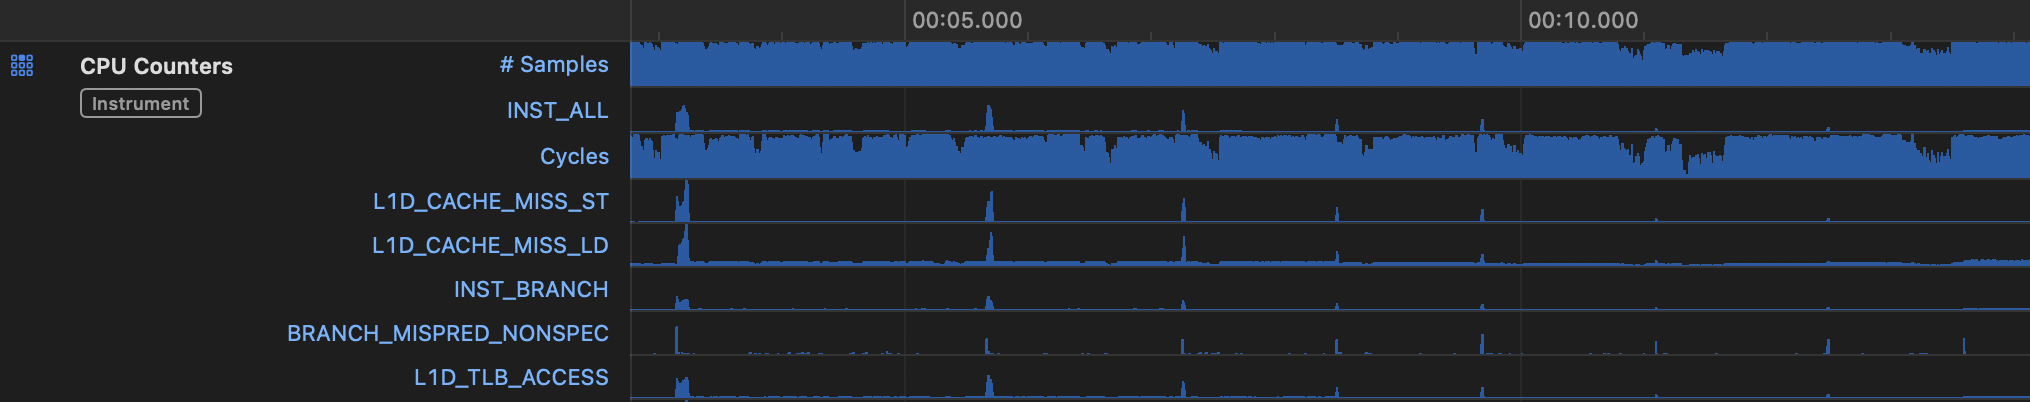
\includegraphics[width=0.75\textwidth]{T2.2.png}
		\caption{Timeline for Cache Line Size Test}
	\end{figure}
	\FloatBarrier
	
	The timeline exhibits distinct periodic spikes while maintaining relatively uniform miss rates in between. These spikes correspond to the initialization and data shuffling (Fisher-Yates) phases at the start of each stride iteration. In earlier steps with smaller stride values, the number of nodes is substantially higher, leading to denser profiling spikes.
	
	Between these setup spikes, cache miss rates remain stable. Because the working dataset is fixed at \textbf{32 MB} (exceeding L2 cache size), fetching data from RAM introduces fixed memory latency bottlenecks, keeping miss density constant. Additionally, the interval between spikes decreases as the stride increases due to the reduction in node count and initialization overhead.
	
	\begin{figure}[h]
		\centering
		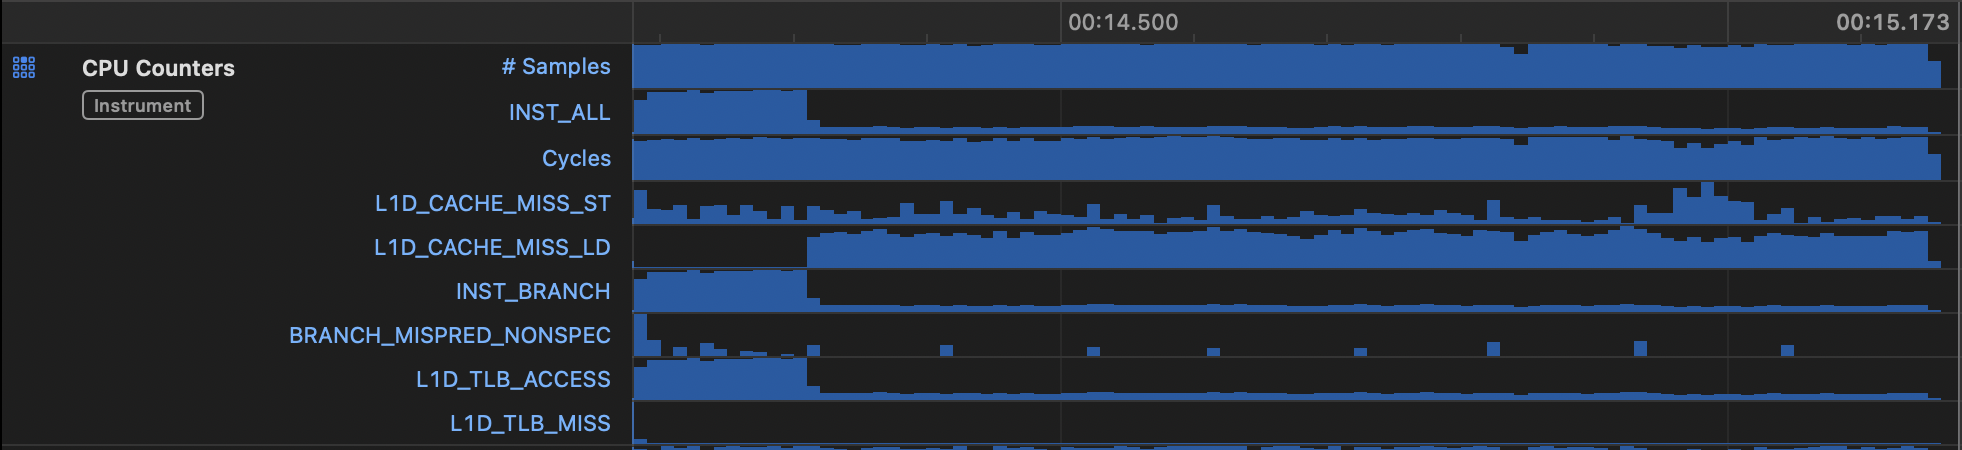
\includegraphics[width=0.75\textwidth]{T2.3.png}
		\caption{Timeline for Set Associativity Test}
	\end{figure}
	\FloatBarrier
	
	At lower associativity degrees, all accessed addresses fit within a single cache set, yielding very few cache misses. Once the number of concurrent pointers exceeds the degree of set associativity ($N > 8$), items can no longer coexist in the set simultaneously. This triggers continuous eviction cycles and a dramatic surge in cache misses.
	
	
	\section{Part 3: Analysis and Optimization of a Performance Phenomenon}
	\textbf{Investigated Phenomenon: Row-Major vs. Column-Major Matrix Traversal}
	
	\subsection{Hypothesis}
	Since multi-dimensional array elements are stored contiguously in memory in row-major order (C-style), row-major traversal is expected to exhibit lower cache miss rates and execution latency compared to column-major traversal, owing to spatial locality.
	
	\subsection{Experiment and Analysis}
	To evaluate this phenomenon, a test program was created using a $4096 \times 4096$ matrix of 4-byte integers. Row-major traversal computes \texttt{matrix[i * SIZE + j] += i + j;} by iterating over rows in the outer loop, whereas column-major traversal iterates over columns in the outer loop.
	
	The snippet corresponding to column-major traversal is shown below:
	
	\begin{figure}[h]
		\centering
		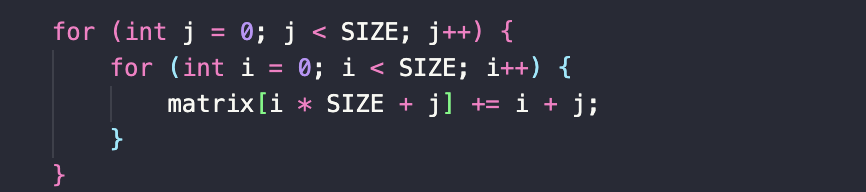
\includegraphics[width=0.75\textwidth]{T3.png}
		\caption{Column-Major Traversal Code Snippet}
	\end{figure}
	\FloatBarrier
	
	The experimental results from the command line interface and Instruments are presented below:
	
	\begin{figure}[h]
		\centering
		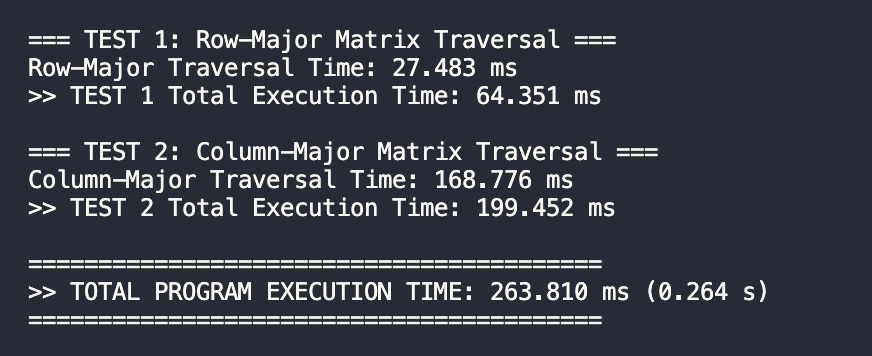
\includegraphics[width=0.75\textwidth]{T3.1.png}
		\caption{Command Line Benchmark Output}
	\end{figure}
	\FloatBarrier
	
	\begin{figure}[h]
		\centering
		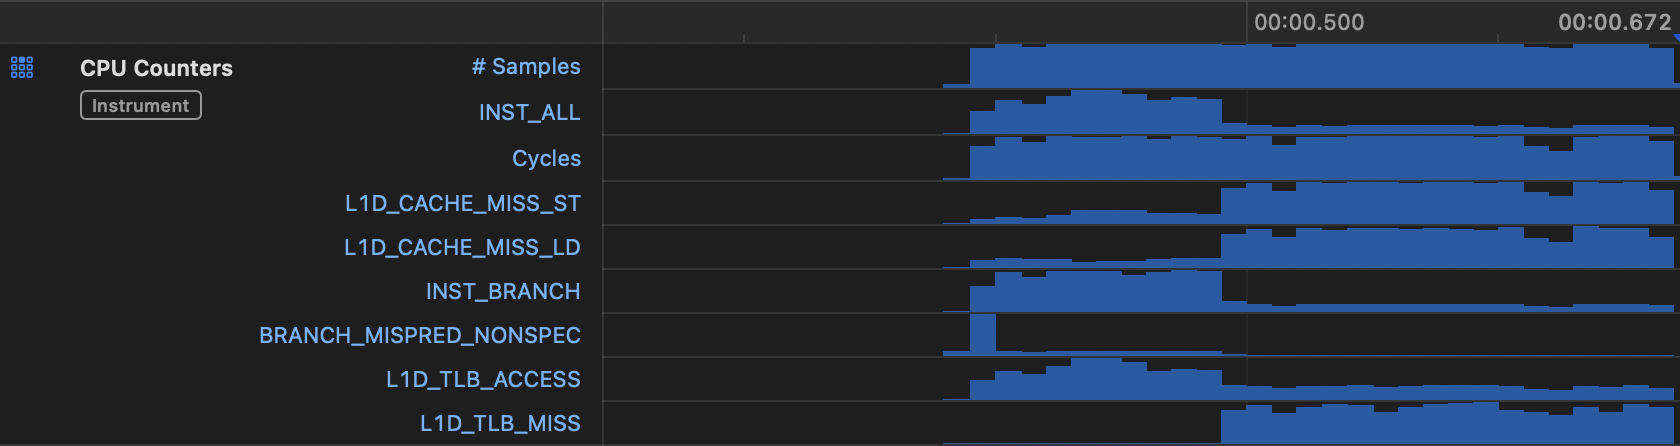
\includegraphics[width=0.75\textwidth]{T3.2.png}
		\caption{Performance Counter Profile in Xcode Instruments}
	\end{figure}
	\FloatBarrier
	
	The column-major traversal exhibits drastically higher execution time and L1 data cache miss rates compared to row-major traversal.
	
	This behavior is directly explained by the principles of spatial locality in cache design. When a cache line is loaded, adjacent memory addresses are fetched into the cache simultaneously. In row-major traversal, contiguous memory accesses benefit from high hit rates because adjacent row elements reside within the same cache line. Conversely, column-major access straddles distinct memory rows (separated by large stride offsets), missing cached data on almost every access and inflating miss density.
	
	\begin{table}[htbp]
		\centering
		\caption{Hardware Counters - Unoptimized (Column-Major)}
		\label{tab:hardware_counters}
		\resizebox{\textwidth}{!}{%
			\begin{tabular}{llllllllll} 
				\toprule
				\textbf{Metric} & \textbf{Samples} & \textbf{INST\_ALL} & \textbf{Cycles} & \textbf{MISS\_ST} & \textbf{MISS\_LD} & \textbf{INST\_BRANCH} & \textbf{MISPRED\_NONSPEC} & \textbf{TLB\_ACCESS} & \textbf{TLB\_MISS} \\
				\midrule
				\textbf{Total} & 2747 & 1,109,406,473 & 516,911,846 & 20,379,099 & 20,228,561 & 260,724,223 & 28,546 & 690,529,492 & 128,591,428 \\
				\bottomrule
			\end{tabular}%
		}
	\end{table}
	
	\subsection{Ruling Out Alternative Hypotheses: Branch Mispredictions}
	One might hypothesize that branch misprediction overhead accounts for the latency disparity in column-major traversal. However, analysis of hardware branch counters reveals that branch mispredictions occur almost exclusively during loop setup and remain negligible throughout execution ($28,546$ mispredictions out of $>260\text{M}$ branch instructions). Thus, branch prediction performance is ruled out as a factor.
	
	
	\subsection{Optimization Strategy: Cache Tiling}
	To mitigate cache misses in column-major traversal, we apply \textbf{Cache Tiling} (blocking). By partitioning the matrix into small sub-blocks of size $32 \times 32$, traversal is confined locally within each tile. Since each tile consumes only $4\,\text{KB}$ of memory (well within L1 capacity), data fits comfortably in cache, dramatically reducing latency.
	
	The hardware counter metrics after applying loop tiling are detailed below:
	
	\begin{table}[htbp]
		\centering
		\caption{Hardware Counters - Optimized (Tiled)}
		\label{tab:hardware_counters_optimized}
		\resizebox{\textwidth}{!}{%
			\begin{tabular}{llllllllll}
				\toprule
				\textbf{Metric} & \textbf{Samples} & \textbf{INST\_ALL} & \textbf{Cycles} & \textbf{MISS\_ST} & \textbf{MISS\_LD} & \textbf{INST\_BRANCH} & \textbf{MISPRED\_NONSPEC} & \textbf{TLB\_ACCESS} & \textbf{TLB\_MISS} \\
				\midrule
				\textbf{Total} & 2208 & 1,157,513,145 & 418,807,471 & 10,803,379 & 25,678,832 & 265,005,114 & 42,767 & 661,948,878 & 4,542,589 \\
				\bottomrule
			\end{tabular}%
		}
	\end{table}
	
	\FloatBarrier
	
	Below is a direct comparison between the original and optimized implementations:
	
	\begin{table}[htbp]
		\centering
		\caption{Hardware Counter Metrics Comparison}
		\label{tab:hardware_counters_comparison}
		\resizebox{\textwidth}{!}{%
			\begin{tabular}{lrrr}
				\toprule
				\textbf{Hardware Metric} & \textbf{Original (Unoptimized)} & \textbf{Optimized (Tiled)} & \textbf{Improvement / Change} \\
				\midrule
				\textbf{Execution Time (ms)} & 271.60 & 217.20 & \textbf{-20.0\% (Faster)} \\
				\textbf{Samples} & 2,747 & 2,208 & -19.6\% \\
				\textbf{Total INST\_ALL} & 1,109,406,473 & 1,157,513,145 & +4.3\% (Overhead) \\
				\textbf{Total Cycles} & 516,911,846 & 418,807,471 & \textbf{-19.0\% (Faster)} \\
				\textbf{L1D\_CACHE\_MISS\_ST} & 20,379,099 & 10,803,379 & \textbf{-47.0\% (Reduced)} \\
				\textbf{L1D\_CACHE\_MISS\_LD} & 20,228,561 & 25,678,832 & +26.9\% \\
				\textbf{INST\_BRANCH} & 260,724,223 & 265,005,114 & +1.6\% \\
				\textbf{BRANCH\_MISPRED\_NONSPEC} & 28,546 & 42,767 & +14,221 ($<0.01\%$ total) \\
				\textbf{L1D\_TLB\_ACCESS} & 690,529,492 & 661,948,878 & -4.1\% \\
				\textbf{L1D\_TLB\_MISS} & 128,591,428 & 4,542,589 & \textbf{-96.5\% (Massive Drop)} \\
				\bottomrule
			\end{tabular}%
		}
	\end{table}
	\FloatBarrier
	
	\subsection{Cross-Sectional Synthesis}
	Based on Part 1 results, the processor cache line size is 128 bytes, meaning each cache line fill fetches 128 bytes into L1 cache. In unoptimized column-major traversal of a $4096 \times 4096$ matrix, traversing a single column spans $4096 \times 128\,\text{bytes} = 512\,\text{KB}$. Given that the processor's L1 Data Cache capacity is $128\,\text{KB}$, traversing a column completely evicts earlier cache lines before they can be reused, inducing severe thrashing. Tiling prevents this eviction cycle, resulting in a **96.5\% reduction in TLB misses** and a **20\% speedup in execution time**.
	
\end{document}
